\documentclass[tikz,border=10pt]{standalone}
\usepackage{tikz}
\usetikzlibrary{positioning,shapes.geometric,arrows.meta,fit,backgrounds}

\begin{document}
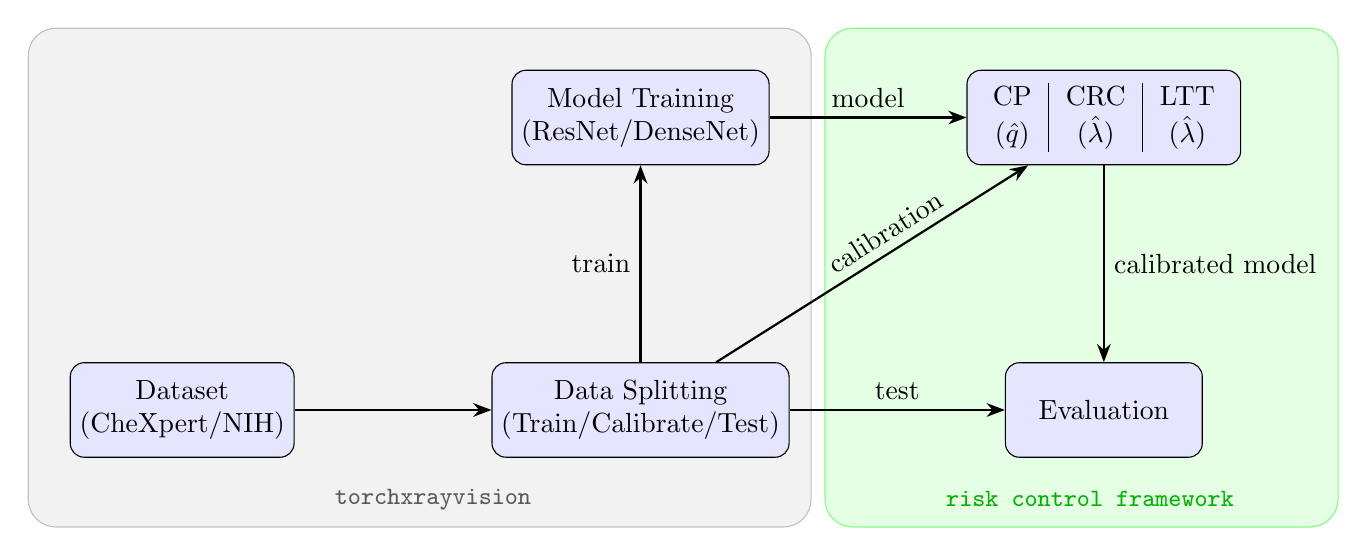
\begin{tikzpicture}[
    node distance=2.5cm,
    box/.style={rectangle, draw, rounded corners=5pt, minimum width=2.5cm, minimum height=1.2cm, align=center, fill=blue!10},
    arrow/.style={-Stealth, thick}
]

% Define nodes - zigzag pattern
\node[box] (dataset) {Dataset\\(CheXpert/NIH)};
\node[box, right=of dataset] (splitting) {Data Splitting\\(Train/Calibrate/Test)};
\node[box, above=of splitting] (training) {Model Training\\(ResNet/DenseNet)};

% Single frameworks node with separators
\node[box, right=of training] (frameworks) {\begin{tabular}{c|c|c}
CP & CRC & LTT \\
\((\hat{q})\) & \((\hat{\lambda})\) & \((\hat{\lambda})\)
\end{tabular}};

\node[box, below=of frameworks] (evaluation) {Evaluation};

\begin{scope}[on background layer]
    \draw[draw=gray!50, fill=gray!10, rounded corners=10pt]
        ([xshift=15pt,yshift=15pt]training.north east) rectangle
        ([xshift=-15pt,yshift=-25pt]dataset.south west);

    \draw[draw=green!50, fill=green!10, rounded corners=10pt]
        ([xshift=35pt,yshift=15pt]frameworks.north east) rectangle
        ([xshift=-65pt,yshift=-25pt]evaluation.south west);
\end{scope}

\node[gray!70!black, font=\small\ttfamily] at ([xshift=-75pt,yshift=-15pt]splitting.south) {torchxrayvision};
\node[green!70!black, font=\small\ttfamily] at ([xshift=-5pt,yshift=-15pt]evaluation.south) {risk control framework};

% Draw arrows
\draw[arrow] (dataset) -- (splitting);
\draw[arrow] (training) -- node[midway, above] {model} (frameworks);
\draw[arrow] (frameworks) -- node[midway, right] {calibrated model} (evaluation);

% Additional arrows from data splitting
\draw[arrow] (splitting) -- node[midway, left] {train} (training);
\draw[arrow] (splitting) -- node[midway, above, sloped, xshift=10pt] {calibration} (frameworks);
\draw[arrow] (splitting) -- node[midway, above, sloped] {test} (evaluation);

\end{tikzpicture}
\end{document}
